\documentclass[a4paper]{article}

\usepackage[english]{babel}
\usepackage[utf8]{inputenc}
\usepackage{amsmath}
\usepackage{graphicx}
\usepackage[numbered]{bookmark}
\usepackage[colorinlistoftodos]{todonotes}
\usepackage{algorithm}
\usepackage{algpseudocode}
\usepackage{pifont}
\usepackage{tikz}
\usepackage{pgfplots}
\usepackage{bm}

\DeclareGraphicsExtensions{.eps,.pdf,.png,.tikz}
\graphicspath{{figs/}}

\title{Coherent Detection Systems for Data Centers}

\author{JKP}

\date{\today}

\begin{document}
\maketitle

\section{Transmitter}
\subsection{Intensity Noise}
Intensity noise is modeled as an AWGN added to the optical power at the transmitter.

The value of the relative intensity noise (RIN) is defined as the ratio between the noise power divide by the noise bandwidth and the signal power \cite{agilent-RIN-measurement}: 
\begin{equation}
RIN = \frac{P_{noise}}{B_{noise}P_{signal}}
\end{equation}

Hence, the \textbf{one-sided RIN PSD} and \textbf{RIN variance} at a certain instant are given by
\begin{align}
& S_{RIN}(t) = RIN\cdot P(t)^2 \\
& \sigma^2_{RIN}(t) = S_{RIN}(t)\frac{f_{s, sim}}{2}
\end{align}
where $f_{s, sim}$ is the sampling frequency to simulate continuous time. Obviously, the variance as defined here only make sense in simulations. Since the intensity noise is assumed to be white, it'd have infinite variance.

Output optical power $P(t)$ is given by
\begin{equation}
P(t) = P_s(t) + w_{RIN}(t)
\end{equation}
where $P_s(t)$ is the signal-only optical power (after modulator frequency response and extinction ratio), and $w_{RIN}(t)\sim\mathcal{N}(0, \sigma^2_{RIN}(t))$.

\subsection{Phase Noise}
Phase noise is modeled as a Wiener process (Gaussian-distributed independent increments).

\begin{equation}
\phi(t+\tau) - \phi(t) \sim\mathcal{N}(0, 2\pi\Delta\nu\tau),
\end{equation} 
where $\Delta\nu$ is the laser linewidth. 

The coherence time is defined as a delay difference yielding an rms value for the phase change of $\sqrt{2}$ rads.

The one-sided PSD of the phase noise is given by
\begin{equation}
	S_{PN}(f) = \frac{\Delta\nu}{\pi f^2}, f > 0.
\end{equation}

\subsection{Modulator Bandwidth Limitations}

\subsubsection{Mach-Zenhder modulator}
\cite{Barros2009, Ho2005}

Limited by loss and velocity mismatch

\begin{equation}
H_{mod}(f) = \frac{1-e^{-\alpha(f)L+j2\pi fd_{12}L}}{\alpha(f)L-j2\pi fd_{12}L}
\end{equation}
where $\alpha(f)$ is the frequency-dependent loss, $d_{12}$ is the velocity mismatch between the optical and electrical waveguides, and $L$ is the interaction length.

\begin{equation}
d_{12} = \frac{n_m-n_r}{c}
\end{equation}
where $n_r \approx 2.15$ is the refractive index of the coplanar waveguide for TM input light. If $n_m$ is only $95\%$ of $n_r$ a significant reduction in bandwidth may occur due to velocity mismatch \cite{Ho2005}.

\subsubsection{Modulator limited by parasitics}
This modulator is modeled as a critically damped second-order system. This is based on the assumption that parasitics capacitances and inductances are the limiting factor in the bandwidth of these devices.

Second-order system with unit damping:
\begin{equation}
H_{mod}(f) =  \frac{1}{1 + 2jf/f_c - (f/f_c)^2}
\end{equation}

The modulator bandwidth is related to $f_c$ by
\begin{equation}
f_{3dB} = \sqrt{\sqrt{2}-1}f_c = 0.64359f_c
\end{equation}

Group delay:
\begin{equation}
\Delta\tau_g = \frac{2}{2\pi f_c}
\end{equation}

\section{Fiber Propagation}
\subsection{Chromatic Dispersion}
\begin{equation}
H(f; L) = \frac{E(f; L)}{E(f, 0)} = e^{-1/2\beta_2(2\pi f)^2L}
\end{equation}
where $H(f; L)$ is fiber frequency response due to dispersion after $L$ meters, and $\beta_2 = -\frac{D(\lambda)\lambda^2}{2\pi c}$. 

Fiber attenuation can be included with the factor $e^{-\frac{1}{2}\frac{att(\lambda)L}{10^4}}$, where $att(\lambda)$ is the fiber attenuation at wavelength $\lambda$ in dB/km.

For SMF28 the fiber dispersion is specified in terms of the zero-dispersion ($\lambda_0$) wavelength and the dispersion slope ($S_0$):
\begin{equation}
D(\lambda) = \frac{S_0}{4}\bigg(\lambda - \frac{\lambda_0^4}{\lambda^3}\bigg), 1200~\text{nm} < \lambda < 1600~\text{nm}
\end{equation}
where $\lambda_0 = 1310$ nm and $S_0 = 0.092$ ps/nm.

\subsection{Polarization Mode Dispersion}
Following \cite{Ip2008}

The output $\bm{y}(t)$ after fiber propagation is given by
\begin{equation}
\bm{r}(t) = \bm{h}(t)\ast \bm{x}(t) + \bm{n}(t)
\end{equation}
where, $\bm{x}(t) = [x_1(t), x_2(t)]^T$, $\bm{n}(t) = [n_1(t), n_2(t)]^T$ and $\bm{h}(t)$ is the matrix representation of the fiber impulse response
\begin{equation}
\bm{h}(t) = \begin{bmatrix}
h_{11}(t) & h_{12}(t) \\
h_{21}(t) & h_{22}(t) \\
\end{bmatrix}
\end{equation}
In the frequency domain for first-order PMD
\begin{equation}
\bm{H}(\omega) = \bm{R}(-\theta)\bm{D}(\omega)\bm{R}(\theta)=\begin{bmatrix}
\cos\theta & -\sin\theta \\
\sin\theta & \cos\theta
\end{bmatrix}\begin{bmatrix}
e^{j\omega\tau_{DGD}/2} & 0 \\
0 & e^{-j\omega\tau_{DGD}/2}
\end{bmatrix}\begin{bmatrix}
\cos\theta & \sin\theta \\
-\sin\theta & \cos\theta
\end{bmatrix}
\end{equation}

The first matrix from the right rotates the input polarization state to the principal states of polarization (PSPs). The second matrix adds a differential group dealy (DGD) $\tau_{DGD}$ between the two PSPs. Finally, the last matrix from the right rotates the PSPs to the output state of polarization.

$\tau_{DGD}$ has a Maxwellian distribution whose mean $\bar{\tau}_{DGD}$ grows with the square of the fiber length. In SMF, typically, $\bar{\tau}_{DGD} = 0.1 \mathrm{ps/\sqrt{km}}$ \cite{Ip2008}. This value assumes the strongly coupled regime, which should be accurate for fibers larger than tens of meters.

This formulation can model both CD and PMD of any order. In simulation, we do CD and PMD separately, since for modeling PMD the fiber has to be broken into small sections.

Hence the fiber propagation is modeled in the frequency domain as
\begin{equation}
\bm{Y}(\omega) = \Big(\bm{H_N}(\omega)\ldots \bm{H_1}(\omega)\Big)\times e^{-\frac{1}{2}\beta_2\omega^2L}
\end{equation}
where each of the $N$ sections of the fiber has frequency response matrix $\bm{H_i}(\omega)$ with a random phase $\theta_i \in [-\pi, \pi]$.
\section{Receiver}
\subsection{Homodyne downconversion}
The received signal electric field $E_s(t)$ and the local oscillator electrical field $E_{LO}(t)$ have the following passband representation
\begin{align}
E_s(t) &= \mathrm{Re}\Big\{\sqrt{2}A_s(t)\exp\Big(j(\omega_st + \phi_{pn}(t))\Big)\Big\} \\
E_{LO}(t) &= \mathrm{Re}\Big\{\sqrt{2}A_{LO}(t)\exp\Big(j(\omega_{LO}t + \phi_{LO}(t))\Big)\Big\}
\end{align}
where $A_s(t)$ and $A_{LO}(t)$ are the complex baseband envelope of the signal and local oscillator electric field, respectively. $\omega_s$ and $\omega_{LO}$ the carrier frequency of the signal and local oscillator electric field. $\phi_s(t)$ is the phase information. $\phi_{pn}(t)$ and $\phi_{LO}(t)$ are the phase noise components.

Hence, it follows that the baseband representation is 
\begin{align}
E_s(t) &= A_s(t) \\
E_{LO}(t) &= A_{LO}(t)\exp\Big(j(\omega_{off}t + \phi_{ph}(t))\Big)
\end{align}
where $\omega_{off} =\omega_{LO}-\omega_s$, and now $\phi_{ph}(t)$ is the phase noise due to LO and transmitter laser combined. For a QPSK signal, $A_s(t) = e^{j\phi_s} = \{e^{j\pi/4}, e^{j3\pi/4}, e^{j5\pi/4}, e^{j7\pi/4}\}$

Considering that the 3-dB coupler has the following transfer matrix
\begin{equation}
\begin{bmatrix}
E_{out, 1} \\
E_{out, 2}
\end{bmatrix} = \frac{1}{\sqrt{2}}\begin{bmatrix}
1 & j \\
j & 1 \\
\end{bmatrix}\begin{bmatrix}
E_{in, 1} \\
E_{in, 2}
\end{bmatrix}
\end{equation}
the $90^o$ hybrid has the following transfer matrix
\begin{equation}
\begin{bmatrix}
E_1\\
E_2\\
E_3\\
E_4
\end{bmatrix} = \frac{1}{2}\begin{bmatrix}
1 & 1 \\
j & -j \\
j & -1\\
-1 & j
\end{bmatrix}\begin{bmatrix}
E{s} \\
E_{LO}
\end{bmatrix}
\end{equation}
where $E_1, E_2, E_3, E_4$ are the input electric fields to the photodiodes.

After balanced detection we have
\begin{align}
I_i(t) = |A_s(t)||A_{LO}(t)|\cos(w_{off}t + \phi_s(t) + \phi_{pn}(t)) \\
I_q(t) = |A_s(t)||A_{LO}(t)|\sin(w_{off}t + \phi_s(t) + \phi_{pn}(t))
\end{align}

Generalizing to the case of \textbf{two polarizations}:
\begin{align}
I_i(t) = \frac{1}{p}|A_s(t)||A_{LO}(t)|\cos(w_{off}t + \phi_s(t) + \phi_{pn}(t)) \\
I_q(t) = \frac{1}{p}|A_s(t)||A_{LO}(t)|\sin(w_{off}t + \phi_s(t) + \phi_{pn}(t))
\end{align}
where $p = 2$ if two polarizations, $p = 1$ otherwise. Note that this convention assumes that the energy per symbol per polarization is 1.  

Therefore, the signal power per real dimension for a quaternary signal is
\begin{align} \nonumber
P_{s} &= \langle|I_i(t)|^2\rangle = \langle|I_q(t)|^2\rangle \\
&= \frac{R^2P_{rx}P_{LO}}{2p^2}
\end{align}
since $P_{rx} = \langle|A_s(t)|^2\rangle$, and $P_{LO} = \langle|A_{LO}(t)|^2\rangle$

One-sided PSD per real dimension of thermal and shot noise:
\begin{align}
S_{th} &= N_0 \\
S_{sh} &= 2(2qRP_{PD})
\end{align}
where $N_0$ is the PSD of the trans-impedance amplifier, the factor of 2 appears due to balance photodetection, and $P_{PD}$ is the incident power in each photodiode:
\begin{equation}
P_{PD} = |E_1|^2 = |E_2|^2 = |E_3|^2 = |E_4|^2 \approx \frac{P_{LO}}{4p}
\end{equation}

%\subsection{Using coherent detection to obtain intensity in a pre-amplified system}
%
%Balanced detectors output:
%\begin{align} \nonumber
%I_I &= |E_1|^2 - |E_2|^2 \\ \nonumber
%&= \frac{1}{2}\Big(E_sE_{LO}^* + E_s^*E_{LO} \Big)
%\end{align}
%
%\begin{align} \nonumber
%I_Q &= |E_3|^2 - |E_4|^2 \\ \nonumber
%&= \frac{1}{2}\Big(-jE_sE_{LO}^* + jE_s^*E_{LO}\Big)
%\end{align}
%
%\begin{align} \nonumber
%Y &= |I_I|^2 + |I_Q|^2 \\ \nonumber
%&= |E_sE_{LO}|^2
%\end{align}
%
%Including noise
%\begin{align} \nonumber
%Y &= |E_sE_{LO}|^2 = |(E_s + E_N)E_{LO}|^2 \\
%&= |E_{LO}|^2(|E_s|^2 + |E_N|^2 + E_s^*E_N + E_sE_N^*) \\
%&= |E_{LO}|^2(|E_s|^2 + |E_N|^2 + 2E_{N,1}\mathrm{Re}(E_s) + 2E_{N,1}\mathrm{Im}(E_s)) \\
%\end{align}

\subsection{SNR calculation}
For real baseband signals we have the following ralations
\begin{equation}
\mathrm{SNR} = \frac{2E_s}{N_0} = \frac{2kE_b}{N_0}
\end{equation}
where $N_0$ is the one-sided real noise PSD, and $k = \log_2(M)$. The factor of 2 relating SNR and $E_s/N_0$ is due to the fact that the two-sided matched filter noise bandwidth of a signal with symbol rate $R_s$ is $R_s$.

For a complex signal, 
\begin{equation}
\mathrm{SNR} = \frac{P_s}{\sigma_n^2} = \frac{E_sR_s}{N_0R_s} = \frac{E_s}{N_0}
\end{equation}
Note that the noise variance is $N_0R_s$ because now the noise has two dimensions. Hence, the one-sided PSD of the complex noise is $2N_0$.

\begin{equation}
\mathrm{SNR} = \frac{E_s}{N_0} = \frac{kE_b}{N_0}
\end{equation}

In both cases $N_0$ denotes the one-sided noise PSD per dimension. 

Hence, the SNR of an ideal system with no intersymbol interfence and employing matched filtering is 
\begin{align} \nonumber
\mathrm{SNR} & = \frac{P_{sig}}{(S_{sh} + S_{th})R_s/2} \\ \nonumber
&= \frac{R^2P_{rx}P_{LO}}{2p^2((2qRP_{LO})/p + N_0)R_s/2} \\
&\approx \frac{RP_{rx}}{pqR_s} 
\end{align}
$R_s$ is the symbol rate and $R_s/2$ is the one-sided noise bandwidth. Note that in this calculation we used the signal power and noise power per real dimension.

\section{PLL-based carrier phase recovery}

\subsection{Phase Locked Loop}

At instant $k$ the symbol $Y_k$ has phase components $\phi_s(k) + \phi_p(k) + \phi_n(k)$, where $\phi_s(k)$ is the signal component and  $\phi_p(k), \phi_n(k)$ are the noise components due to phase noise and additive Gaussian noise, respectively. $\phi_p(k)$ is a Weiner process whose random steps have variance $2\pi(2\nu)T_s$, where $\nu$ is the laser linewidth of both transmitter laser and local oscillator. $T_s$ is the symbol period. $\phi_n(k)$ has a von Mises also known as circular normal distribution or Tikhonov distribution.

\begin{equation} \label{eq:Tikhonov-pdf}
	\phi_n(k) \sim p(x; \mu, \kappa) = \frac{1}{2\pi I_0(\kappa)}\exp(\kappa\cos(x-\mu))
\end{equation}
where $\mu, 1/\kappa$ are analogous to $\mu$ $\sigma^2$ in the normal distribution. $I_0(\kappa)$ si the modified Bessel function of order 0.

Assuming that the phase estimation process perfectly removes the signal component from the phase of $Y_k$, the input to the PLL filter is $\phi_p(k) + \phi_n(k)$.

Note: the distribution of the ratio of two zero-mean Gaussian random variable is a Cauchy random variable.

\subsection{Loop Filter}
Second-order loop filter
\begin{equation}
F(s) = \frac{2\xi\omega_ns + \omega_n^2}{s},
\end{equation}
where $\xi$ is the damping factor, which is typically $\xi = \sqrt{2}/2$, and $\omega_n$ is the relaxation frequency, which must be optimized in order to reduce the phase error variance.

Including the integrator from the VCO
\begin{equation}
G(s) = \frac{2\xi\omega_ns + \omega_n^2}{s^2}
\end{equation}

Hence, the impulse response $sG(s)$ in time-domain is given by
\begin{equation}
g(t) = 2\xi\omega_nu(t) + \omega_n^2tu(t)
\end{equation}

\subsubsection{Continuous time}

The open-loop response of the PLL is given by
\begin{equation}
G(s) = \frac{F(s)}{s}e^{-s\Delta_T}
\end{equation}
where $\Delta_T$ is the loop delay, which includes group delay of the filters as well as propagation delays. $G(s)$ is the transfer function between the local oscillator phase and the phase noise, which also includes AWGN component. 

When there's a frequency offset in addition to a phase error, the input to the PLL is a ramp. Hence, from the final value theorem we can determine the steady-state phase error
\begin{equation}
	\phi_e(t\to\infty) = \lim_{s\to 0} \frac{sR(s)}{1 + G(s)} = \lim_{s\to 0}s\frac{1}{s^2}\cdot\frac{s^2}{s^2 + 2\xi\omega_ns + \omega_n^2} = 0
\end{equation}
Therefore, in continuous-time, a PLL has zero error to a frequency offset.

\subsubsection{Discrete time}

We can obtain the open-loop transfer function by discretizing the continuous-time transfer function $G(s)$, either using a bilinear transformation or impulse invariance.

From bilinear transformation
\begin{equation}
	G(z) = \frac{z^2(\xi\omega_nT_s + T_s^2\omega_n^2/4) + 2zT_s^2\omega_n^2/4 + T_s^2\omega_n^2/4 - \xi\omega_nT_s}{z^2 - 2z + 1} = \frac{P(z)}{(z-1)^2}
\end{equation}

Applying the final value theorem to a ramp input
\begin{align} \nonumber
	\phi_e(n\to\infty) &= \lim_{z\to 1} \frac{(z-1)\frac{(z)}{(z-1)^2}}{1 + G(z)} = \lim_{z\to 1} \frac{z}{(z-1)(1 + G(z))} \\
	&= \lim_{z\to 1} \frac{z(z-1)}{(z-1)^2 + P(z)} = 0
\end{align}
Hence, the DPLL implementation also achieves zero error for a ramp input i.e., frequency offset. However, since the delay in the phase estimation of an actual implementation of a DPLL is at least 1, the output constellation will be rotated by at least $f_{off}/R_s$ radians.

\subsection{Homodyne detection}
After balanced detection we have in each polarization
\begin{align}
I_i(t) = R\frac{\sqrt{P_{rx}P_{LO}}}{p}\cos(w_{off}t + \phi_s(t) + \phi_{pn}(t)) \\
I_q(t) =  R\frac{\sqrt{P_{rx}P_{LO}}}{p}\sin(w_{off}t + \phi_s(t) + \phi_{pn}(t))
\end{align}

After phase detection using a Costas loop, we have

\begin{equation}
S(t) = R\frac{\sqrt{2P_{rx}P_{LO}}}{p}\sin(\phi_{pn}(t)) + n_i(t) + n_q(t)
\end{equation}

Using the small-signal approximation $\sin x \approx x$:
\begin{equation}
S(t) \approx R\frac{\sqrt{2P_{rx}P_{LO}}}{p}\phi_{pn}(t) + n_i(t) + n_q(t)
\end{equation}

The phase error of the OPLL $\phi_e(t)$ is related to the phase noise $\phi_{pn}(t)$ by

\begin{equation} \label{eq:phase-error-in-s}
\phi_e(s) = N_{CPR}\frac{s}{s + F(s)e^{-s\tau_d}}\phi_{pn}(s) - \frac{F(s)e^{-s\tau_d}}{s + F(s)e^{-s\tau_d}}n(s)
\end{equation}
where $n(s) \sim\mathcal{N}(0, 2N_{CPR}\sigma_n^2)$, $N_{CPR}$ is the number of polarizations used in carrier phase recovery, and $F(s) = 2\zeta\omega_n + \omega_n^2/s$, for a second-order loop filter. Note that \eqref{eq:phase-error-in-s} assumes that there's no mismatch from the phase noise estimate of the two polarizations. The mismatch case will be analyzed in the next subsection.

Defining the phase estimation gain
\begin{equation}
K_D = N_{CPR}R\frac{\sqrt{2P_{rec}P_{LO}}}{p}
\end{equation}

If all noise contributions are assumed ergodic:
\begin{equation}
\sigma_E^2 = E\{\phi_e(t)\}
\end{equation}

Since the system is linear
\begin{align} \label{eq:phase_error_variance} \nonumber
\sigma_E^2 &= E\{\phi_n^2(t)\} + E\{\phi_{AWGN}(t)^2\} \\ \nonumber
&= \frac{1}{2\pi}\int_{-\infty}^\infty S_{PN}(f)\bigg|\frac{j\omega}{j\omega + F(j\omega)e^{-j\omega\tau_d}}\bigg|^2d\omega + \frac{1}{2\pi K_D^2}\int_{-\infty}^\infty S_{AWGN}(f)\bigg|\frac{F(j\omega)}{j\omega + F(j\omega)e^{-j\omega\tau_d}}\bigg|^2d\omega \\ \nonumber
&= \Delta\nu_{TOT}\int_{-\infty}^\infty \bigg|\frac{1}{j\omega + F(j\omega)e^{-j\omega\tau_d}}\bigg|^2d\omega + \frac{2N_0/2N_{CPR}}{2\pi K_D^2}\int_{-\infty}^\infty \bigg|\frac{F(j\omega)}{j\omega + F(j\omega)e^{-j\omega\tau_d}}\bigg|^2d\omega \\
&= \Delta\nu_{TOT}\int_{-\infty}^\infty \bigg|\frac{1}{j\omega + F(j\omega)e^{-j\omega\tau_d}}\bigg|^2d\omega + \frac{1}{2\pi 2N_{CPR}\gamma_sR_s}\int_{-\infty}^\infty \bigg|\frac{F(j\omega)}{j\omega + F(j\omega)e^{-j\omega\tau_d}}\bigg|^2d\omega 
\end{align}
where $S_{PN}(f) = \frac{\Delta\nu}{2\pi f^2}$, where $\Delta\nu$ is the combined laser linewidth of the transmitter laser and LO.  $\Delta\nu$ is the full-width half-maximum of the Lorentzian shape of phase noise PSD. $N_0$ is the AWG noise one-sided PSD per real dimension. $\gamma_s$ is the SNR.

\subsection{Costas loop analysis with skew between two polarizations}

In the previous section, it was assumed that the phase noise estimate $\phi_{pn}(t)$ were perfectly synchronized. Here, we'll assume that the phase noise from the Y polarization is delayed from the phase noise estimate from the X polarization by $\Delta t$. That is,

\begin{align}
\phi_{pn, X}(t) &= \phi_{pn}(t) \\
\phi_{pn, Y}(t)& = \phi_{pn}(t-\Delta t) = \phi_{pn}(t) - \phi_{\Delta t},
\end{align}
where $\phi_{\Delta t} \sim \mathcal{N}(0, 2\pi\Delta\nu_{tot}\Delta t)$, since phase noise is assumed to be a Wiener process.

\begin{equation}
S(t) \approx R\frac{\sqrt{2P_{rx}P_{LO}}}{p}(2\phi_{pn}(t) - \phi_{\Delta t}) + n(t),
\end{equation}
where $n(t) \sim\mathcal{N}(0, 4\sigma_n^2)$. The 4 factor appears due to I, Q and from the two polarizations. Note that $\sigma_n^2$ already includes a factor of 2 due to balanced photodetection. 

Now the phase error of the PLL has an additional component due to the mismatch between the two polarizations
\begin{equation}
\phi_e(s) = \frac{s}{s + F(s)e^{-s\tau_d}}\phi_{pn}(s) - \frac{s}{s + F(s)e^{-s\tau_d}}\phi_{\Delta t}(s) - \frac{F(s)e^{-s\tau_d}}{s + F(s)e^{-s\tau_d}}n(s)
\end{equation}

\begin{align} \nonumber
\sigma_E^2 &= \Delta\nu_{TOT}\int_{-\infty}^\infty \bigg|\frac{1}{j\omega +  F(j\omega)e^{-j\omega\tau_d}}\bigg|^2d\omega \\
& + \frac{2\pi\Delta\nu\Delta t}{4} t\lim_{\Omega\to\infty}\frac{1}{\Omega}\int_{-\Omega}^\Omega \bigg|\frac{j\omega}{j\omega +  F(j\omega)e^{-j\omega\tau_d}}\bigg|^2d\omega \\
&+ \frac{1}{2\pi 4\gamma_sR_s}\int_{-\infty}^\infty \bigg|\frac{F(j\omega)}{j\omega + F(j\omega)e^{-j\omega\tau_d}}\bigg|^2d\omega \nonumber
\end{align}

Assuming that the integral in the middle term is approximately one, then the additional phase error variance due to mismatch is $\frac{2\pi\Delta\nu\Delta t}{4}$. This only becomes considerable if the mismatch $\Delta t$ is in the order of hundreds of symbols.

Assuming now that only the X polarization is used in the carrier phase recovery, but the Y polarization is delay from the X polarization by $\Delta t$.

\begin{align} \nonumber
\sigma_E^2 &= \Delta\nu_{TOT}\int_{-\infty}^\infty \bigg|\frac{1}{j\omega +  F(j\omega)e^{-j\omega\tau_d}}\bigg|^2d\omega \\
& + 2\pi\Delta\nu\Delta t \lim_{\Omega\to\infty}\frac{1}{\Omega}\int_{-\Omega}^\Omega \bigg|\frac{j\omega}{j\omega +  F(j\omega)e^{-j\omega\tau_d}}\bigg|^2d\omega \\
&+ \frac{1}{2\pi 2\gamma_sR_s}\int_{-\infty}^\infty \bigg|\frac{F(j\omega)}{j\omega + F(j\omega)e^{-j\omega\tau_d}}\bigg|^2d\omega \nonumber
\end{align}

In this case the error due to the skew between the two polarization is $2\pi\Delta\nu\Delta t$.

\subsection{Effect of flicker noise}

Flicker noise or $1/f$ noise is a frequency noise due to fluctuations on the laser temperature. Fig.~\ref{fig:freq_noise_psd} illustrates the laser frequency noise PSD \cite{Kazovsky1986}.

The one-sided PSD of the phase noise is given by
\begin{align}
S_{PN}(f) = \frac{\Delta\nu}{\pi f^2} \\
S_{1/f}(f) = \frac{k_a}{f^3}
\end{align}
where the first term is the phase noise PSD due to the Lorentzian-shape linewidth, and the second is due to flicker noise.

According to \cite{Fatadin2013}, $k_a = 1.7\times 10^{11}~\mathrm{Hz}^2$ for an integrated tunable laser with nearly 911 kHz linewidth, and $k_a = 0.75\times 10^{10}~\mathrm{Hz}^2$ for a DFB with nearly 300 kHz linewidth. Note that the variable $s_1$ defined in \cite[equation (3)]{Fatadin2013} is related to $k_a$ by $k_a = s_1/2$ because here we use double-sided PSD of the phase noise.

Adding another term to \ref{eq:phase_error_variance} due to flicker noise yields

\begin{align} \label{eq:phase_error_variance_flicker} \nonumber
\sigma_E^2 &= \Delta\nu_{TOT}\int_{-\infty}^\infty \bigg|\frac{1}{j\omega + F(j\omega)e^{-j\omega\tau_d}}\bigg|^2d\omega \\ \nonumber
&+ 2(2\pi)^2 k_a\int_{0}^\infty \frac{1}{\omega}\bigg|\frac{1}{j\omega + F(j\omega)e^{-j\omega\tau_d}}\bigg|^2d\omega \\
&+ \frac{1}{2\pi 2N_{CPR}\gamma_sR_s}\int_{-\infty}^\infty \bigg|\frac{F(j\omega)}{j\omega + F(j\omega)e^{-j\omega\tau_d}}\bigg|^2d\omega 
\end{align}

\begin{figure} [!t]
	\centering
	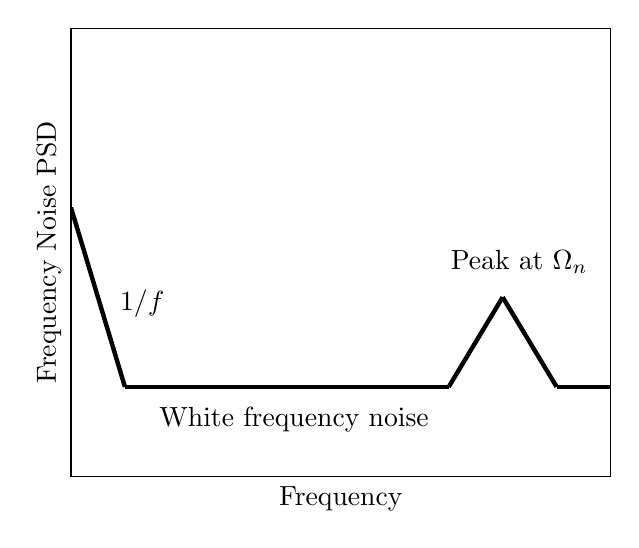
\begin{tikzpicture}
\begin{axis}[
xmin=0,
xmax=10,
ymin=0,
ymax=5, 
xlabel=Frequency,
ylabel=Frequency Noise PSD,
ticks=none,
samples=10]
\addplot[black, ultra thick, domain=1:7] (x, 1);
\addplot[black, ultra thick, domain=0:1] (x, 3-2*x);
\addplot[black, ultra thick, domain=7:8] (x, x-6);
\addplot[black, ultra thick, domain=8:9] (x, -x+10);
\addplot[black, ultra thick, domain=9:10] (x, 1);
\end{axis}     
\draw (0.5, 2.5) node [below right] {$1/f$};
\draw (4.7, 3) node [below right] {Peak at $\Omega_n$};
\draw (1, 1) node [below right] {White frequency noise};
\end{tikzpicture}
	\caption{Laser Frequency Noise PSD. Three components are illustrated: (i) low-frequency flicker noise with slope $1/f$ in the logarithmic graph due temperature fluctuations of the laser, (ii) white phase noise associated with the Lorentzian linewidth of the laser, and (iii) a peak at the laser resonance frequency $\omega_n$. This last term is negligible since this peak occurs at tens of GHz, which is much larger than the loop filter bandwidth \cite{Kazovsky1986}.} \label{fig:freq_noise_psd}
\end{figure}

\subsection{Comparison between phase noise and AWGN components of phase error variance}

Both the phase noise and the AWGN component in the phase error variance have a denominator given by $|j\omega + F(j\omega)e^{-j\omega\tau_d}|$, where $F(j\omega) = 2\zeta\omega_n - j\omega_n^2/\omega$. The phase error will grow unbounded whenever this denominator goes to zero. Equating the real and complex parts of the denominator
\begin{align}
-\omega^2 + 2\zeta\omega_n\omega\sin(\omega\tau_d) + \omega_n^2\cos(\omega\tau_d) = 0 \\
2\zeta\omega_n\omega\cos(\omega\tau_d) - \omega_n^2\sin(\omega\tau_d) = 0
\end{align}
Using the small-signal approximations $\sin(x)\approx x$ and $\cos(x) \approx 1$. We have
\begin{align}
2\zeta\omega_n\tau_d = 1 - (\omega_n/\omega)^2 \\
2\zeta = \omega_n\tau_d
\end{align}

The solution of the second equation $\omega_n = \frac{2\zeta}{\tau_d}$. In simulations, we use $\omega_{n, \max} = \frac{\zeta}{\tau_d}$.


\subsection{PLL terminology}
Sections extracted from \cite{Gardner} chapters 5 and 8. 

\subsubsection{Hold-in range}
Frequency range over which the loop will hold lock. In other words, the largest step in frequency over which the system will still hold lock.	

\subsubsection{Lock-in range (self-acquisition range)}

If signal frequency is close enough to VCO frequency, a PLL locks up with
just a phase transient; there is no cycle slipping prior to lock. The frequency range over which the loop acquires phase without slips is called the lock-in range of the PLL. In a first-order loop, the lock-in range is equal to the hold-in range; the loop self-acquires any signal that it can hold. The same is not true of type 2 or higher loops; \textbf{the lock-in range is invariably less than the hold-in range}. Moreover, there is a frequency interval, smaller than the hold-in interval
and larger than the lock-in interval, over which the loop will acquire lock after slipping cycles for awhile. This intermediate interval is called the pull-in range.

\subsubsection{Frequency pull-in, or simply, pull-in}

Pull-in Limits If the loop filter contains a perfect integrator, pull-in will be accomplished no matter how large the initial frequency error. (This statement neglects clipping limits; the loop clearly cannot pull in a signal that requires excessive control voltage to the VCO. Also, it is assumed that there are no unwanted DC offsets within the loop that would counteract the pull-in voltage and cause the VCO frequency to be pushed out instead.) In an analog loop filter, the integrator is imperfect and the DC gain is some finite number F(0). If vp is small enough—if the initial frequency error is large enough—the loop cannot pull in. The largest frequency for which the loop can still pull into lock is called the pull-in limit and is represented by $\Delta\omega_p$.

\begin{figure}[h!]
	\centering
	\includegraphics[width=\textwidth]{transient_phase_error_of_2nd_order_pll.png}
	\label{fig:transient_2nd_pll}
	\caption{\cite{Gardner}}
\end{figure}

There is some frequency-step limit below which the loop does not slip cycles but remains in lock; denote this limit as the \textbf{pullout frequency}

\section{Digital signal processing}

\subsection{Fractionally spaced linear equalizer}

Long-haul systems typically have a static equalization stage to compensate for CD and a dynamic equalization stage, which is adapted more often since PMD changes over time.

For this application bandwidth limitations due to modulator and other devices, chromatic dispersion, polarization-mode dispersion are assumed to be small enough so they can all be compensated by a single equalization stage. 

Assuming an oversampling ratio $r_{os} = p/q$, $p, q \in \mathrm{Z^*_+}$, which need not be integer, we can compensate for inter-symbol interference (ISI) and demultiplex the two polarizations.

Samples at the equalizer input $\bm{X}[k]$, where $x_1[k], x_2[k]$ are the complex samples from the two polarizations. $k$ is at a rate $T_s/r_{os}$.

The equalizer output can be written as
\begin{align}
\hat{x}_{1}[k] = w^{(i)}_{11}[k]\ast x_1[k] + w^{(i)}_{12}[k]\ast x_2[k] \\
\hat{x}_{2}[k] = w^{(i)}_{21}[k]\ast x_1[k] + w^{(i)}_{22}[k]\ast x_2[k]
\end{align}

where $i = 1, \ldots, q$. We need a total of $q$ filters because in the case of non-interger oversampling ratio the samples do not align. For instance, If $r_{os} = 3/2$, we need two sets of filters, one for the odd samples and another for the even samples.

This can be simplified if DGD is small so that 

\begin{align}
\hat{x}_{1}[k] = w^{(i)}_{1}[k]\ast x_1[k] + w_{21}^{(i)}w^{(i)}_{2}[k]\ast x_2[k] \\
\hat{x}_{2}[k] = w^{(i)}_{2}[k]\ast x_2[k] + w_{12}^{(i)}w^{(i)}_{1}[k]\ast x_1[k]
\end{align}
where $i = 1, \ldots, q$. Note that in this case we only have two filters $w^{(i)}_{1}$ and $w^{(i)}_{2}$ per symbol. The terms $w_{21}^{(i)}$ and $w_{12}^{(i)}$ are cross terms, which are also determined adaptively. Hence the number of operations is approximately halved.

The number of required is sufficiently small that time-domain equalization is less complex than frequency-domain equalization.

\subsection{Constant Modulus Algorithm}

Constant Modulus Algorithm (CMA) is a blind equalization algorithm that relies on the fact that PSK or 4-QAM constellations have a constant modulus. 

For being a blind algorithm, CMA cannot separate the symbols. If there's a fixed phase error CMA will converge to that phase offset. If there's a mismatch between the transmitter and local oscillator, the CMA output will rotate at a rate that is the difference between the two frequencies. For this reason, the constellation diagram after CMA is typically a circle. 


\subsection{Frequency Recovery}
\cite{Hoffmann2008} 

Input signal is in the form

\begin{equation}
x[k] = x_ke^{j2\pi\Delta fk + \phi[k]}
\end{equation}
where $\Delta f$ is the frequency offset to be estimated.

\begin{equation}
\Delta f[k] = \Delta f[k](1-\mu) + \mu\frac{\mathrm{arg}\{(x[k]x^*[k-1]^4)\}}{8\pi T_s}
\end{equation}
where $\mu$ is adaptation constant and $T_s$ is the symbol time. The $\mathrm{arg}\{\cdot\}$ function may require unwrapping to prevent cycle slips. Biased unwrapping, which takes into account estimated frequency was shown to have better performance \cite{Hoffmann2008}.

\subsection{Phase Tracking}
\cite{Phase1995}

Given the signal $y[k]$ after CMA equalization. The phase tracking algorithm applies a phase shift $z(k) = y[k]e^{-j\Phi[k]}$, where
\begin{equation}
\Phi[k+1] = \Phi[k]-\mu\mathrm{Im}\{z[k]e^*[k]\}
\end{equation}
where $e^*[k] = z[k] - \hat{x}[k]$, where $\hat{x}[k]$ is a decision made based on $z[k]$.


\section{DPSK}
\subsection{Frequency offset penalty}

In DPSK symbols the transmitted information is encoded as phase changes. In comparison with coherent PSK, DPSK has an inherent penalty of 2.4 dB.

To simplify the receiver the DPSK receiver design, we will assume that the receiver does not do any form of frequency carrier recovery. 

The receiver decodes the signal by determining the phase transitions between consecutive symbols. Phase noise, AWGN, and frequency offset lead to phase error. While phase noise is negligible between two symbols, frequency offset between transmitter laser and LO may lead to significant error. The error probability of M-DSPK signals was studied by \cite{Pawula2001}. The bit error probability for a DPSK signal in the presence of frequency offset is given by

\begin{equation}
P_e \approx \frac{2}{\log_2M}(F(\pi) - F(\pi/M)),
\end{equation}
where
\begin{equation}
F(\phi) = \frac{\gamma_s\sin(\Delta\Psi-\phi)}{4\pi}\int_{-\pi/2}^{\pi/2} \frac{\exp(-(\gamma_s -\gamma_s\cos(\Delta\Psi - \phi)\cos t))}{\gamma_s -\gamma_s\cos(\Delta\Psi - \phi)\cos t}dt
\end{equation}
and 
\begin{equation}
\Delta\Psi = 2\pi f_{off}T_s
\end{equation}
is the frequency offset.

This equation assumes that the SNR between two symbols is the same.

\section{QPSK phase error with imperfect carrier phase recovery}
Following \cite{Prabhu1976}, the bit error probability of a QPSK system with imperfect carrier phase recovery so that the residual phase error $\epsilon$ is such that $\epsilon \sim \mathcal{N}(\mu_\epsilon, \sigma_\epsilon^2)$ is given by
\begin{equation}
P_b = \frac{1}{2}\mathrm{erfc}(\sqrt{\rho}) + \sum_{l = 0}^\infty (-1)^lH_l\Big(1 - \cos((2l+1)\pi/4)\cos((2l+1)\mu_\epsilon)\exp(-(2l+1)^2\sigma_\epsilon^2)\Big)
\end{equation}
where
\begin{equation}
H_l = \frac{\rho\exp(-\rho^2/2)}{\sqrt{\pi}(2l+1)}\Big(I_l(\rho^2/2) + I_{l+1}(\rho^2/2)\Big)
\end{equation}
where $rho$ denotes the SNR, and $I_l(x)$ is the modified Bessel function of first kind.


\section{DBR lasers}

According to \cite[Section III]{Ristic2010} there are at least four important characteristics that make SG-DBR attractive for its use in an OPLL.

\begin{enumerate}
	\item ``SG-DBR lasers have in excess of 40 nm of quasi-continuous wavelength tuning range''
	
	This advantage is not that important in a communication system. It's not important for an initial demonstration. 
	
	\item ``the FM tuning mechanism of the SG-DBR laser is very efficient. Unlike Distributed Feedback (DFB) lasers, which are tuned by current injection into the laser gain section, in SG-DBR lasers, the tuning is achieved by current injection into a small, separate, passive phase section.''
	
	This advantage no longer exists for a multi-electrode DFB.
	
	\item ``Third, an important advantage of the SG-DBR laser is that, unlike in a typical DFB laser, there is no sign change in its FM phase response. The FM response has a 3 dB bandwidth of 70 MHz, and no phase inversion is observed below this frequency. The phase inversion in a DFB laser occurs within its bandwidth at a frequency where the thermal effect becomes too slow to dominate frequency tuning with the corresponding red shift in the FM response so that frequency tuning becomes dominated by the carrier-injection effect and the corresponding blue shift in the FM response. It is very challenging to implement an OPLL feedback electronic circuit that can compensate for this phase inversion. The absence of phase inversion in the FM phase response of an SG-DBR laser is due to the fact that: 1) the small and efficient phase tuning pads require small currents for tuning, thereby reducing the thermal effects and 2) the phase section is composed of the passive material that has a band gap larger than that of the active material so that the accumulation of carriers is very efficient as they cannot be depleted by stimulated emission. ''
	
	This problem no longer exists in multi-electrode DFB lasers \cite{Jacquet1993}.
	
	\item ``Fourth, the linewidth of an SG-DBR laser is dominated by low-frequency jitter [39], which is not very difficult to compensate with the large bandwidth of an integrated OPLL, which as we will show below is at least 300 MHz.'' 
	
	This may actually be undesirable since we would like to make the loop frequency smaller.
	
\end{enumerate}

From \cite{Langley1999}
``Standard current-tuned lasers have an FM response dominated by thermal effects at low frequencies, giving a red-shifting response with increasing current, while at high frequencies, the response is dominated by band-filling and plasma effects, giving a blue-shifting response [63], [64].''

The LO laser must have a FM response that is dominated by carrier injection even at low frequencies. 

The FM response of standard DFB lasers is dominated by thermal effects up to 0.1 MHz, and after that carrier injection becomes the dominant effect. These two mechanisms have opposite frequency shifts, which leads to a dip in the FM response. For this application, thermal effects must be minimized so that the FM response is flat up to a few GHz and primarily caused by carrier injection. This is typically achieve with multi-electrode DFB lasers .

\cite{Dilwali1992}
Empirical Thermal FM
\begin{equation}
H_{TH}(f) = -\frac{2K_T}{3\sqrt{\frac{jf}{f_c}}}\Big[\tanh\Big(\frac{jf}{f_c}\Big)^{\frac{1}{2}} + \tanh\Big(\frac{1}{2}\Big(\frac{jf}{f_c}\Big)^\frac{1}{2}\Big)\Big]
\end{equation}
where $K_T$ is the thermal FM gain, which increases with the bias.

Carrier-induced FM
\begin{equation}
H_{CFM}(\omega) = K_c\frac{1 + j\omega\omega_m/\omega_0^2}{1 - (\omega/\omega_0)^2 + j(\omega/\omega_0)}
\end{equation}
where $K_c$ is the efficiency at low frequencies in HzmA$^{-1}$, $\omega_0$ is the bias-dependent relaxation oscillation frequency, and $\omega_m = \tau_1\omega_0^2$, where $\tau_1$ is a damping time constant.

Note that while the thermal FM has a negative sign (red shift), the carrier-induced FM has a positive sign (blue shift). This leads to a dip in the FM response once the thermal FM decays at higher frequencies. Moreover, this sign change is undesirable, since in practice it would require some form of equalization.




\bibliographystyle{plain}
\bibliography{bib}

\end{document}